\section{strlen()}
\index{\CStandardLibrary!strlen()}

\RU{Ещё немного о циклах. Часто функция \TT{strlen()}\footnote{подсчет длины строки в Си} 
реализуется при помощи \TT{while()}.}
\EN{Let's talk about loops one more time. Often, the \TT{strlen()} 
function\footnote{counting the characters in a string in the C language} is implemented using a \TT{while()} 
statement.}
\RU{Например, вот как это сделано в стандартных библиотеках MSVC:}
\EN{Here is how it is done in the MSVC standard libraries:}

\lstinputlisting{patterns/10_strings/1_strlen/ex1.c}

% subsections
\subsection{x86}

\subsubsection{\NonOptimizing MSVC}

\RU{Итак, компилируем:}\EN{Let's compile:}

\lstinputlisting{patterns/10_strings/1_strlen/10_1_msvc.asm.\LANG}

\index{x86!\Instructions!MOVSX}
\index{x86!\Instructions!TEST}
\RU{Здесь две новых инструкции: \MOVSX и \TEST.}
\EN{We get two new instructions here: \MOVSX and \TEST.}

\label{MOVSX}
\RU{О первой. \MOVSX предназначена для того, чтобы взять байт из какого-либо места в памяти и положить его, 
в нашем случае, в регистр \EDX. 
Но регистр \EDX~--- 32-битный. \MOVSX означает \IT{MOV with Sign-Extend}. 
Оставшиеся биты с 8-го по 31-й \MOVSX сделает единицей, если исходный байт в памяти имеет знак \IT{минус}, 
или заполнит нулями, если знак \IT{плюс}.}
\EN{The first one---\MOVSX---takes a byte from an address in memory and stores the value in a 32-bit register. 
\MOVSX stands for \IT{MOV with Sign-Extend}. 
\MOVSX sets the rest of the bits, from the 8th to the 31th, 
to 1 if the source byte is \IT{negative} or to 0 if is \IT{positive}.}

\RU{И вот зачем всё это.}\EN{And here is why.}

\RU{По умолчанию в MSVC и GCC тип \Tchar~--- знаковый. Если у нас есть две переменные, одна \Tchar, а другая \Tint 
(\Tint тоже знаковый), и если в первой переменной лежит -2 (что кодируется как \TT{0xFE}) и мы просто 
переложим это в \Tint, 
то там будет \TT{0x000000FE}, а это, с точки зрения \Tint, даже знакового, будет 254, но никак не -2. 
-2 в переменной \Tint кодируется как \TT{0xFFFFFFFE}. Для того чтобы значение \TT{0xFE} из переменной типа 
\Tchar переложить 
в знаковый \Tint с сохранением всего, нужно узнать его знак и затем заполнить остальные биты. 
Это делает \MOVSX.}
\EN{By default, the \Tchar type is signed in MSVC and GCC. If we have two values of which one is \Tchar 
and the other is \Tint, (\Tint is signed too), and if the first value contain -2 (coded as \TT{0xFE}) 
and we just copy this byte into the \Tint container, it makes \TT{0x000000FE}, and this 
from the point of signed \Tint view is 254, but not -2. In signed int, -2 is coded as \TT{0xFFFFFFFE}. 
So if we need to transfer \TT{0xFE} from a variable of \Tchar type to \Tint, 
we need to identify its sign and extend it. That is what \MOVSX does.}

\RU{См. также об этом раздел}
\EN{You can also read about it in} \q{\IT{\SignedNumbersSectionName}}\EN{ section}~(\myref{sec:signednumbers}).

\RU{Хотя конкретно здесь компилятору вряд ли была особая надобность хранить значение \Tchar в регистре \EDX, 
а не его восьмибитной части, скажем \DL. Но получилось, как получилось. Должно быть 
\gls{register allocator} компилятора сработал именно так.}
\EN{It's hard to say if the compiler needs to store a \Tchar variable in \EDX, it could just take a 8-bit register part 
(for example \DL). Apparently, the compiler's \gls{register allocator} works like that.}

\index{ARM!\Instructions!TEST}
\RU{Позже выполняется \TT{TEST EDX, EDX}. 
Об инструкции \TEST читайте в разделе о битовых полях~(\myref{sec:bitfields}).
Конкретно здесь эта инструкция просто проверяет состояние регистра \EDX на 0.}
\EN{Then we see \TT{TEST EDX, EDX}. 
You can read more about the \TEST instruction in the section about bit fields~(\myref{sec:bitfields}).
Here this instruction just checks if the value in \EDX equals to 0.}

\ifdefined\IncludeGCC
\subsubsection{\NonOptimizing GCC}

\RU{Попробуем}\EN{Let's try} GCC 4.4.1:

\lstinputlisting{patterns/10_strings/1_strlen/10_3_gcc.asm}

\label{movzx}
\index{x86!\Instructions!MOVZX}
\RU{Результат очень похож на MSVC, только здесь используется \MOVZX, а не \MOVSX. 
\MOVZX означает \IT{MOV with Zero-Extend}. Эта инструкция перекладывает какое-либо значение 
в регистр и остальные биты выставляет в 0.
Фактически, преимущество этой инструкции только в том, что она позволяет 
заменить две инструкции сразу: \TT{xor eax, eax / mov al, [...]}.}
\EN{The result is almost the same as in MSVC, but here we see \MOVZX instead of \MOVSX. 
\MOVZX stands for \IT{MOV with Zero-Extend}. 
This instruction copies a 8-bit or 16-bit value into a 32-bit register and sets the rest of the bits to 0. 
In fact, this instruction is convenient only because it enable us to replace this instruction pair: 
\TT{xor eax, eax / mov al, [...]}.}

\RU{С другой стороны, нам очевидно, что здесь можно было бы написать вот так: 
\TT{mov al, byte ptr [eax] / test al, al}~--- это тоже самое, хотя старшие биты \EAX будут \q{замусорены}. 
Но будем считать, что это погрешность компилятора~--- 
он не смог сделать код более экономным или более понятным. 
Строго говоря, компилятор вообще не нацелен на то, чтобы генерировать понятный (для человека) код.}
\EN{On the other hand, it is obvious that the compiler could produce this code: 
\TT{mov al, byte ptr [eax] / test al, al}---it is almost the same, however, 
the highest bits of the \EAX register will contain random noise. 
But let's think it is compiler's drawback---it cannot produce more understandable code. 
Strictly speaking, the compiler is not obliged to emit understandable (to humans) code at all.}

\index{x86!\Instructions!SETcc}
\RU{Следующая новая инструкция для нас~--- \SETNZ. В данном случае, если в \AL был не ноль, 
то \TT{test al, al} выставит флаг \ZF в 0, а \SETNZ, если \TT{ZF==0} 
(\IT{NZ} значит \IT{not zero}) выставит 1 в \AL. 
Смысл этой процедуры в том, что 
\IT{если AL не ноль, выполнить переход на} \TT{loc\_80483F0}.
Компилятор выдал немного избыточный код, но не будем забывать, что оптимизация выключена.}
\EN{The next new instruction for us is \SETNZ. 
Here, if \AL doesn't contain zero, \TT{test al, al} 
sets the \ZF flag to 0, but \SETNZ, if \TT{ZF==0} (\IT{NZ} stands for \IT{not zero}) sets \AL to 1.
Speaking in natural language, \IT{if \AL is not zero, let's jump to loc\_80483F0}. 
The compiler emits some redundant code, but let's not forget that the optimizations are turned off.}
\fi

\subsubsection{\Optimizing MSVC}
\label{strlen_MSVC_Ox}

\RU{Теперь скомпилируем всё то же самое в MSVC 2012, но с включенной оптимизацией (\Ox)}
\EN{Now let's compile all this in MSVC 2012, with optimizations turned on (\Ox)}:

\lstinputlisting[caption=\Optimizing MSVC 2012 /Ob0]{patterns/10_strings/1_strlen/10_2.asm.\LANG}

\RU{Здесь всё попроще стало. Но следует отметить, что компилятор обычно может так хорошо использовать регистры 
только на небольших функциях с небольшим количеством локальных переменных.}
\EN{Now it is all simpler.
Needless to say, the compiler could use registers with such efficiency
only in small functions with a few local variables.}

\index{x86!\Instructions!INC}
\index{x86!\Instructions!DEC}
\INC/\DEC\EMDASH\RU{это инструкции \glslink{increment}{инкремента}-\glslink{decrement}{декремента}. Попросту говоря~--- 
увеличить на единицу или уменьшить.}
\EN{are \gls{increment}/\gls{decrement} instructions, in other words: add or substract 1 to/from a variable.}

\ifdefined\IncludeOlly
\clearpage
\subsubsection{\Optimizing MSVC + \olly}
\index{\olly}

\RU{Можем попробовать этот (соптимизированный) пример в}
\EN{We can try this (optimized) example in} \olly.
\RU{Вот самая первая итерация}\EN{Here is the first iteration}:

\begin{figure}[H]
\centering
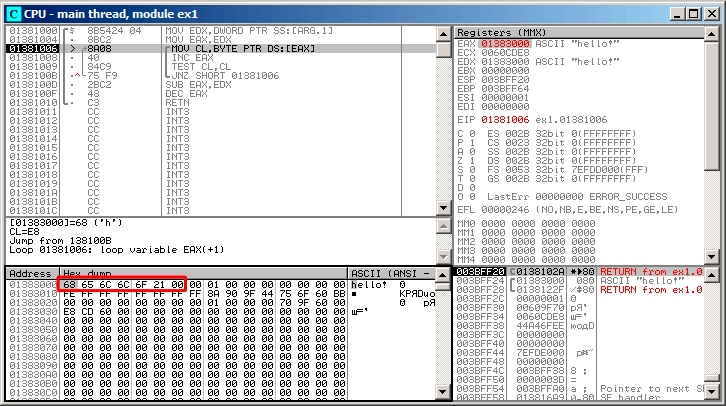
\includegraphics[scale=\FigScale]{patterns/10_strings/1_strlen/olly1.png}
\caption{\olly: \RU{начало первой итерации}\EN{first iteration start}}
\label{fig:strlen_olly_1}
\end{figure}

\RU{Видно, что \olly обнаружил цикл и, для удобства, \IT{свернул} инструкции тела цикла в скобке.}
\EN{We see that \olly found a loop and, for convenience, \IT{wrapped} its instructions in brackets.}
\RU{Нажав правой кнопкой на}\EN{By clicking the right button on} \EAX, \RU{можно выбрать}\EN{we can choose} 
\q{Follow in Dump} 
\RU{и позиция в окне памяти будет как раз там, где надо.}
\EN{and the memory window scrolls to the right place.}
\RU{Здесь мы видим в памяти строку}\EN{Here we can see the string} \q{hello!}\EN{ in memory}.
\RU{После неё имеется как минимум 1 нулевой байт, затем случайный мусор}\EN{There is at least
one zero byte after it and then random garbage}.
\RU{Если \olly видит, что в регистре содержится адрес какой-то строки, он показывает эту строку.}
\EN{If \olly sees a register with a valid address in it, that points to some string, 
it is shown as a string.}

\clearpage
\RU{Нажмем}\EN{Let's press} F8 (\stepover) \RU{столько раз, чтобы текущий адрес снова был 
в начале тела цикла}\EN{a few times, to get to the start of the body of the loop}:

\begin{figure}[H]
\centering
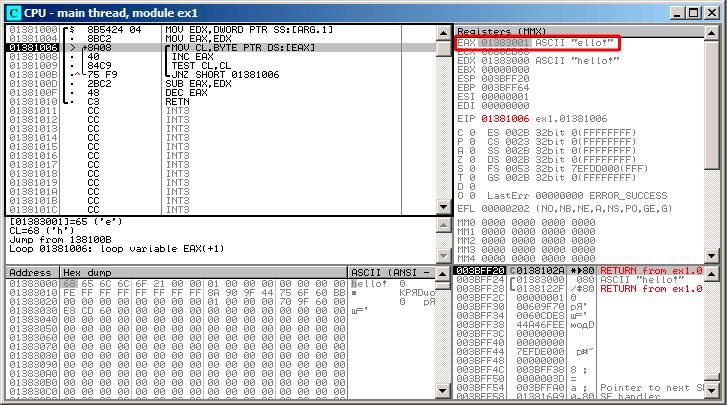
\includegraphics[scale=\FigScale]{patterns/10_strings/1_strlen/olly2.png}
\caption{\olly: \RU{начало второй итерации}\EN{second iteration start}}
\label{fig:strlen_olly_2}
\end{figure}

\RU{Видно, что}\EN{We see that} \EAX \RU{уже содержит адрес второго символа в строке.}
\EN{contains the address of the second character in the string.}

\clearpage
\RU{Будем нажимать F8 достаточное количество раз, чтобы выйти из цикла:}
\EN{We have to press F8 enough number of times in order to escape from the loop:}

\begin{figure}[H]
\centering
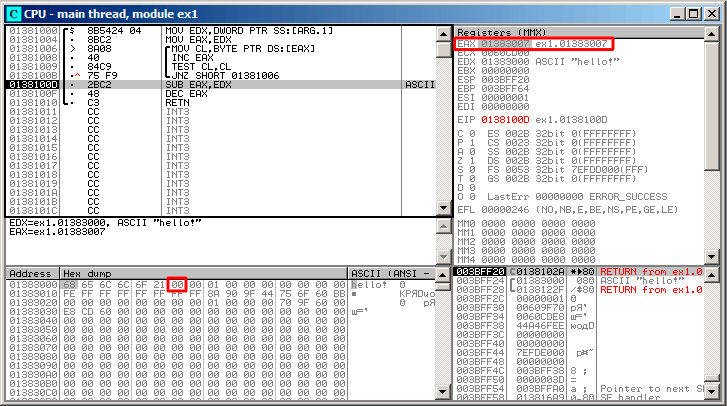
\includegraphics[scale=\FigScale]{patterns/10_strings/1_strlen/olly3.png}
\caption{\olly: \RU{сейчас будет вычисление разницы указателей}\EN{pointers difference to be calculated now}}
\label{fig:strlen_olly_3}
\end{figure}

\RU{Увидим, что \EAX теперь содержит адрес нулевого байта, следующего сразу за строкой.}
\EN{We see that \EAX now contains the address of zero byte that's right after the string.}
\RU{А \EDX так и не менялся~--- он всё ещё указывает на начало строки}\EN{Meanwhile, \EDX hasn't changed,
so it still pointing to the start of the string}.
\RU{Здесь сейчас будет вычисляться разница между этими двумя адресами.}
\EN{The difference between these two addresses is being calculated now.}

\clearpage
\RU{Инструкция \SUB исполнилась}\EN{The \SUB instruction just got executed}:

\begin{figure}[H]
\centering
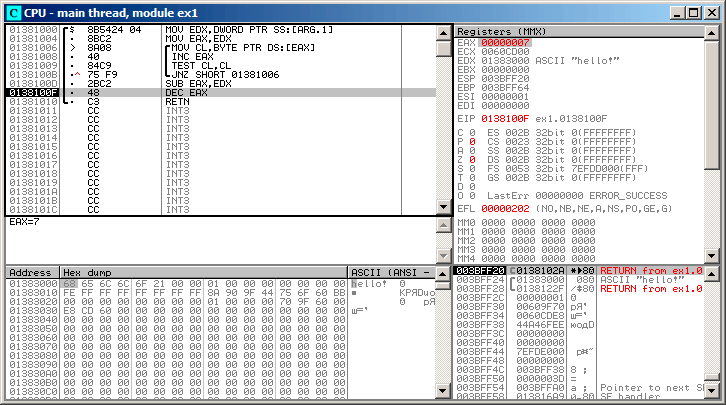
\includegraphics[scale=\FigScale]{patterns/10_strings/1_strlen/olly4.png}
\caption{\olly: \RU{сейчас будет декремент \EAX}\EN{\EAX to be decremented now}}
\label{fig:strlen_olly_4}
\end{figure}

\RU{Разница указателей сейчас в регистре \EAX~--- 7.}
\EN{The difference of pointers is in the \EAX register now---7.}
\RU{Действительно, длина строки}\EN{Indeed, the length of the} \q{hello!}\RU{~--- 6}\EN{ string is 6}, 
\RU{но вместе с нулевым байтом}\EN{but with the zero byte included}\EMDASH{}7.
\RU{Но}\EN{But} \TT{strlen()} 
\RU{должна возвращать количество ненулевых символов в строке.}
\EN{must return the number of non-zero characters in the string.}
\RU{Так что сейчас будет исполняться декремент и выход из функции.}
\EN{So the decrement executes and then the function returns.}

\fi

\ifdefined\IncludeGCC
\subsubsection{\Optimizing GCC}

\RU{Попробуем GCC 4.4.1 с включенной оптимизацией (ключ \Othree):}
\EN{Let's check GCC 4.4.1 with optimizations turned on (\Othree key):}

\lstinputlisting{patterns/10_strings/1_strlen/10_3_gcc_O3.asm}

\RU{Здесь GCC не очень отстает от MSVC за исключением наличия \MOVZX.} 
\EN{Here GCC is almost the same as MSVC, except for the presence of \MOVZX.}

\RU{Впрочем, \MOVZX здесь явно можно заменить на}
\EN{However, here \MOVZX could be replaced with} \TT{mov dl, byte ptr [eax]}.

\RU{Но возможно, компилятору GCC просто проще помнить, что у него под переменную типа \Tchar отведен целый 
32-битный регистр \EDX и быть уверенным в том, что старшие биты регистра не будут замусорены.}
\EN{Probably it is simpler for GCC's code generator to \IT{remember} 
the whole 32-bit \EDX register 
is allocated for a \Tchar variable and it then can be sure that the highest bits has no any noise 
at any point.}

\label{strlen_NOT_ADD}
\index{x86!\Instructions!NOT}
\index{x86!\Instructions!XOR}
\RU{Далее мы видим новую для нас инструкцию \NOT. Эта инструкция инвертирует все биты в операнде. 
Можно сказать, что здесь это синонимично инструкции \TT{XOR ECX, 0ffffffffh}. 
\NOT и следующая за ней инструкция \ADD вычисляют разницу указателей и отнимают от результата единицу. 
Только происходит это слегка по-другому. Сначала \ECX, где хранится указатель на \IT{str}, 
инвертируется и от него отнимается единица.}
\EN{After that we also see a new instruction---\NOT. This instruction inverts all bits in the operand. 
You can say that it is a synonym to the \TT{XOR ECX, 0ffffffffh} instruction. 
\NOT and the following \ADD calculate the pointer difference and subtract 1, just in a different way. 
At the start \ECX, where the pointer to \IT{str} is stored, gets inverted and 1 is subtracted from it.}

\RU{См. также раздел:}\EN{See also:} \q{\SignedNumbersSectionName}~(\myref{sec:signednumbers}).

\RU{Иными словами, в конце функции, после цикла, происходит примерно следующее:} 
\EN{In other words, at the end of the function just after loop body, these operations are executed:}

\begin{lstlisting}
ecx=str;
eax=eos;
ecx=(-ecx)-1; 
eax=eax+ecx
return eax
\end{lstlisting}

\dots~\RU{что эквивалентно}\EN{and this is effectively equivalent to}:

\begin{lstlisting}
ecx=str;
eax=eos;
eax=eax-ecx;
eax=eax-1;
return eax
\end{lstlisting}

\RU{Но почему GCC решил, что так будет лучше? Трудно угадать.
Но наверное, оба эти варианта работают примерно одинаково в плане эффективности и скорости.}
\EN{Why did GCC decide it would be better? Hard to guess. 
But perhaps the both variants are equivalent in efficiency.}
\fi

\ifdefined\IncludeARM
\subsection{ARM}

% subsubsections
\subsubsection{32-\RU{битный}\EN{bit} ARM}

\myparagraph{\NonOptimizingXcodeIV (\ARMMode)}

\lstinputlisting[caption=\NonOptimizingXcodeIV (\ARMMode),label=ARM_leaf_example7]{patterns/10_strings/1_strlen/ARM/xcode_ARM_O0.asm.\LANG}

\RU{Неоптимизирующий LLVM генерирует слишком много кода. Зато на этом примере можно посмотреть, 
как функции работают с локальными переменными в стеке.}
\EN{Non-optimizing LLVM generates too much code, however, here we can see how the function works with 
local variables in the stack.}
\RU{В нашей функции только локальных переменных две\EMDASH{}это два указателя:}%
\EN{There are only two local variables in our function:}
\IT{eos} \AndENRU \IT{str}.
\RU{В этом листинге сгенерированном при помощи \IDA мы переименовали \IT{var\_8} и \IT{var\_4} в \IT{eos} и \IT{str} вручную.}%
\EN{In this listing, generated by \IDA, we have manually renamed \IT{var\_8} and \IT{var\_4} to \IT{eos} and \IT{str}.}

\RU{Итак, первые несколько инструкций просто сохраняют входное значение в обоих переменных}
\EN{The first instructions just saves the input values into both} \IT{str} \AndENRU \IT{eos}.

\RU{С метки}\EN{The body of the loop starts at label} \IT{loc\_2CB8}\RU{ начинается тело цикла}.

\RU{Первые три инструкции в теле цикла}\EN{The first three instruction in the loop body} (\TT{LDR}, \ADD, \TT{STR}) 
\RU{загружают значение}\EN{load the value of} \IT{eos} \RU{в}\EN{into} \Reg{0}. 
\RU{Затем происходит инкремент значения и оно сохраняется в локальной переменной \IT{eos} расположенной 
в стеке.}\EN{Then the value is \glslink{increment}{incremented} and saved back into \IT{eos}, which is located in the stack.}

\index{ARM!\Instructions!LDRSB}
\RU{Следующая инструкция}\EN{The next instruction, } \TT{LDRSB R0, [R0]} (\q{Load Register Signed Byte}) 
\RU{загружает байт из памяти по адресу \Reg{0}, расширяет его до 32-бит считая его знаковым (signed) 
и сохраняет в \Reg{0}}\EN{, loads a byte from memory at the address stored in \Reg{0} 
and sign-extends it to 32-bit}%
\footnote{\RU{Компилятор Keil считает тип \Tchar знаковым, как и MSVC и GCC}\EN{The Keil compiler 
treats the \Tchar type as signed, just like MSVC and GCC}.}.
\index{x86!\Instructions!MOVSX}
\RU{Это немного похоже на инструкцию}\EN{This is similar to the} \MOVSX \RU{в}\EN{instruction in} x86.
\RU{Компилятор считает этот байт знаковым (signed), потому что тип \Tchar по стандарту Си~--- знаковый.}
\EN{The compiler treats this byte as signed since the \Tchar type is signed according to the C standard.}
\RU{Об этом уже было немного написано}\EN{It was already written about it}~(\myref{MOVSX}) \RU{в этой же секции, 
но посвященной x86}\EN{in this section, in relation to x86}.

\index{Intel!8086}
\index{Intel!8080}
\index{ARM}
\RU{Следует также заметить, что в ARM нет возможности использовать 8-битную или 16-битную часть 
регистра, как это возможно в x86.}
\EN{It has to be noted that it is impossible to use 8- or 16-bit part 
of a 32-bit register in ARM separately of the whole register,
as it is in x86.}
\RU{Вероятно, это связано с тем, что за x86 тянется длинный шлейф совместимости со своими предками, 
вплоть до 16-битного 8086 и даже 8-битного 8080, 
а ARM разрабатывался с чистого листа как 32-битный RISC-процессор.}
\EN{Apparently, it is because x86 has a huge history of backwards compatibility with its ancestors 
up to the 16-bit 8086 and even 8-bit 8080,
but ARM was developed from scratch as a 32-bit RISC-processor.}
\RU{Следовательно, чтобы работать с отдельными байтами на ARM, так или иначе придется использовать 
32-битные регистры.}
\EN{Consequently, in order to process separate bytes in ARM, one has to use 32-bit registers anyway.}

\RU{Итак}\EN{So}, \TT{LDRSB} \RU{загружает символы из строки в \Reg{0}, по одному.}
\EN{loads bytes from the string into \Reg{0}, one by one.}
\RU{Следующие инструкции}\EN{The following} \CMP \AndENRU \ac{BEQ} \RU{проверяют, является ли этот символ 0.}
\EN{instructions check if the loaded byte is 0.}
\RU{Если не 0, то происходит переход на начало тела цикла.}\EN{If it's not 0, control passes to the start
of the body of the loop.}
\RU{А если 0, выходим из цикла.}\EN{And if it's 0, the loop ends.}

\RU{В конце функции вычисляется разница между}\EN{At the end of the function, the difference between} 
\IT{eos} \AndENRU \IT{str}\RU{, вычитается единица, и вычисленное 
значение возвращается через \Reg{0}.}\EN{ is calculated, 1 is subtracted from it, and resulting value is returned
via \Reg{0}.}

N.B. \RU{В этой функции не сохранялись регистры}\EN{Registers were not saved in this function}.
\index{ARM!\Registers!scratch registers}
\RU{По стандарту регистры \Reg{0}-\Reg{3} называются также \q{scratch registers}.
Они предназначены для передачи аргументов и 
их значения не нужно восстанавливать при выходе из функции, потому что они больше не нужны в вызывающей функции.
Таким образом, их можно использовать как захочется.}
\EN{That's because in the ARM calling convention registers \Reg{0}-\Reg{3} are \q{scratch registers}, 
intended for arguments passing,
and we're not required to restore their value when the function exits, 
since the calling function will not use them anymore.
Consequently, they may be used for anything we want.}
\RU{А~так~как никакие больше регистры не используются, то и сохранять нечего.}
\EN{No other registers are used here, so that is why we have nothing to save on the stack.}
\RU{Поэтому управление можно вернуть вызывающей функции 
простым переходом (\TT{BX}) по адресу в регистре \ac{LR}.}
\EN{Thus, control may be returned back to calling function by a simple jump (\TT{BX}),
to the address in the \ac{LR} register.}

%\subsubsection{\NonOptimizingXcodeIV + режим Thumb}
%Практически, точно такой же код.

\myparagraph{\OptimizingXcodeIV (\ThumbMode)}

\lstinputlisting[caption=\OptimizingXcodeIV (\ThumbMode)]{patterns/10_strings/1_strlen/ARM/xcode_thumb_O3.asm}

\RU{Оптимизирующий LLVM решил, что под переменные \IT{eos} и \IT{str} выделять место в стеке не обязательно,}
\EN{As optimizing LLVM concludes, \IT{eos} and \IT{str} do not need space on the stack,}
\RU{и эти переменные можно хранить прямо в регистрах.}
\EN{and can always be stored in registers.}
\RU{Перед началом тела цикла \IT{str} будет находиться в \Reg{0}, 
а \IT{eos}\EMDASH{}в \Reg{1}.}
\EN{Before the start of the loop body, \IT{str} is always in \Reg{0}, 
and \IT{eos}\EMDASH{}in \Reg{1}.}

\index{ARM!\Instructions!LDRB.W}
\EN{The}\RU{Инструкция} \TT{LDRB.W R2, [R1],\#1} \RU{загружает в \Reg{2} байт из памяти по адресу \Reg{1}, 
расширяя его как знаковый (signed), до 32-битного
значения, но не только это.}
\EN{instruction loads a byte from the memory at the address stored in \Reg{1}, to \Reg{2}, sign-extending it to a 32-bit value, but not
just that.}
\RU{\TT{\#1} в конце инструкции означает \q{Post-indexed addressing},
т.е. после загрузки байта к \Reg{1} добавится единица.}
\EN{\TT{\#1} at the instruction's end is implies \q{Post-indexed addressing},
which means that 1 is to be added to \Reg{1} after the byte is loaded.}

\RU{Читайте больше об этом}\EN{Read more about it}: \myref{ARM_postindex_vs_preindex}.

\RU{Далее в теле цикла можно увидеть \CMP и \ac{BNE}. Они продолжают работу цикла до тех пор, 
пока не будет встречен 0.}
\EN{Then you can see \CMP and \ac{BNE} in the body of the loop, these instructions continue looping until
0 is found in the string.}

\index{ARM!\Instructions!MVNS}
\index{x86!\Instructions!NOT}
\RU{После конца цикла }\TT{MVNS}\footnote{MoVe Not} 
\RU{(инвертирование всех бит, \NOT в x86)}
\EN{(inverts all bits, like \NOT in x86)}
\RU{и \ADD вычисляют}\EN{and \ADD instructions compute} $eos - str - 1$.
\RU{На самом деле, эти две инструкции вычисляют}
\EN{In fact, these two instructions compute}
$R0 = ~str + eos$, 
\RU{что эквивалентно тому, что было в исходном коде. Почему это так, уже было описано чуть раньше, здесь}
\EN{which is effectively equivalent to what was in the source code, and why it is so, was already explained here}
~(\myref{strlen_NOT_ADD}).

\RU{Вероятно, LLVM, как и GCC, посчитал, что такой код может быть короче (или быстрее).}
\EN{Apparently, LLVM, just like GCC, concludes that this code can be shorter (or faster).}

%\subsubsection{\OptimizingXcodeIV + \ARMMode}
%Практически, точно такой же код.

\myparagraph{\OptimizingKeilVI (\ARMMode)}

\lstinputlisting[caption=\OptimizingKeilVI (\ARMMode),label=ARM_leaf_example6]{patterns/10_strings/1_strlen/ARM/Keil_ARM_O3.asm}

\index{ARM!\Instructions!SUBEQ}
\RU{Практически то же самое, что мы уже видели, за тем исключением, что выражение}
\EN{Almost the same as what we saw before, with the exception that the}
$str - eos - 1$ 
\RU{может быть вычислено не в самом конце функции, а прямо в теле цикла.}
\EN{expression can be computed not at the function's end, but right in the body of the loop.}
\EN{The}\RU{Суффикс} \TT{-EQ} \RU{означает, что инструкция будет выполнена только
если операнды в исполненной перед этим инструкции \CMP были равны.}
\EN{suffix, as we may recall, implies that the instruction executes only if the operands in
the \CMP that was executed before were equal to each other.}
\RU{Таким образом}\EN{Thus}, \RU{если в \Reg{0} будет 0}\EN{if \Reg{0} contains 0},
\RU{обе инструкции}\EN{both} \TT{SUBEQ} \RU{исполнятся и результат останется в \Reg{0}.}
\EN{instructions executes and result is left in the \Reg{0} register.}


\subsubsection{ARM64}

\myparagraph{\Optimizing GCC (Linaro) 4.9}

\lstinputlisting{patterns/10_strings/1_strlen/ARM/ARM64_GCC_O3.lst.\LANG}

\RU{Алгоритм такой же как и в}\EN{The algorithm is the same as in} \myref{strlen_MSVC_Ox}: 
\RU{найти нулевой байт, затем вычислить разницу между указателями, затем отнять 1 от результата}\EN{find a zero 
byte, calculate the difference between the pointers and decrement the result by 1}.
\RU{Комментарии добавлены автором книги}\EN{Some comments were added by the author of this book}.

\RU{Стоит добавить, что наш пример имеет ошибку: \TT{my\_strlen()}
возвращает 32-битный \Tint, тогда как должна возвращать \TT{size\_t} или иной 64-битный тип.}%
\EN{The only thing worth noting is that our example is somewhat wrong: \TT{my\_strlen()}
returns 32-bit \Tint, while it has to return \TT{size\_t} or another 64-bit type.}

\RU{Причина в том, что теоретически, \TT{strlen()} можно вызывать для огромных блоков в памяти,
превышающих 4GB, так что она должна иметь возможность вернуть 64-битное значение на 64-битной платформе.}
\EN{The reason is that, theoretically, \TT{strlen()} can be called for a huge blocks in memory that exceeds
4GB, so it must able to return a 64-bit value on 64-bit platforms.}
\RU{Так что из-за моей ошибки, последняя инструкция \SUB работает над 32-битной частью регистра, тогда
как предпоследняя \SUB работает с полными 64-битными частями (она вычисляет разницу между указателями).}
\EN{Because of my mistake, the last \SUB instruction operates on a 32-bit part of register, while the penultimate
\SUB instruction works on full the 64-bit register (it calculates the difference between the pointers).}
\RU{Это моя ошибка, но лучше оставить это как есть, как пример кода, который возможен в таком случае.}
\EN{It's my mistake, it is better to leave it as is, as an example of how the code could look like in such case.}

\myparagraph{\NonOptimizing GCC (Linaro) 4.9}

\lstinputlisting{patterns/10_strings/1_strlen/ARM/ARM64_GCC_O0.lst.\LANG}

\RU{Более многословно}\EN{It's more verbose}.
\RU{Переменные часто сохраняются в память и загружаются назад (локальный стек)}\EN{The variables are 
often tossed here to and from memory (local stack)}.
\RU{Здесь та же ошибка: операция декремента происходит над 32-битной частью регистра}\EN{The same mistake here: 
the decrement operation happens on a 32-bit register part}.


\fi
\ifdefined\IncludeMIPS
\subsection{MIPS}

\lstinputlisting[caption=\Optimizing GCC 4.4.5 (IDA)]{patterns/10_strings/1_strlen/MIPS_O3_IDA.lst.\LANG}

\index{MIPS!\Instructions!NOR}
\index{MIPS!\Pseudoinstructions!NOT}
\RU{В MIPS нет инструкции \NOT, но есть \NOR~--- операция \TT{OR~+~NOT}.}
\EN{MIPS lacks a \NOT instruction, but has \NOR which is \TT{OR~+~NOT} operation.}
\RU{Эта операция широко применяется в цифровой электронике\footnote{\NOR называют \q{универсальным элементом}.
Например, космический компьютер Apollo Guidance Computer использовавшийся в программе \q{Аполлон} был
построен исключительно на 5600 элементах \NOR: \cite{Eickhoff}.}, но не очень популярна в программировании.}
\EN{This operation is widely used in digital electronics\footnote{NOR is called \q{universal gate}.
For example, the Apollo Guidance Computer used in the Apollo program, 
was built by only using 5600 NOR gates: \cite{Eickhoff}.}, but isn't very popular in computer programming.}
\RU{Так что операция \NOT реализована здесь как}\EN{So, the NOT operation is implemented here as} 
\TT{NOR~DST,~\$ZERO,~SRC}.

\RU{Из фундаментальных знаний \myref{sec:signednumbers}, мы можем знать, что побитовое инвертирование знакового
числа это то же что и смена его знака с вычитанием 1 из результата.}
\EN{From fundamentals \myref{sec:signednumbers} we know that bitwise inverting a signed number is the same 
as changing its sign and subtracting 1 from the result.}
\RU{Так что \NOT берет значение $str$ и трансформирует его в $-str-1$.}
\EN{So what \NOT does here is to take the value of $str$ and transform it into $-str-1$.}
\RU{Следующая операция сложения готовит результат}\EN{The addition operation that follows prepares result}.

\fi
